\section{Annexe}

\subsection{Images}
\begin{figure}[H]
    \centering
    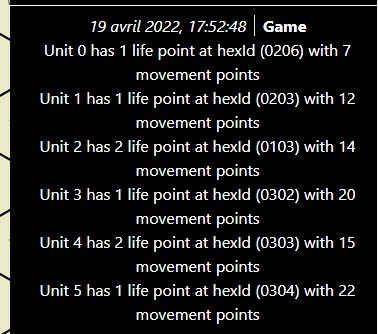
\includegraphics[scale=0.6]{data/info_units.jpg}
    \caption{Terminal qui donne les informations des unités du joueur 1 }.
    \label{fig:units_command}
\end{figure}

\begin{figure}[H]
    \centering
    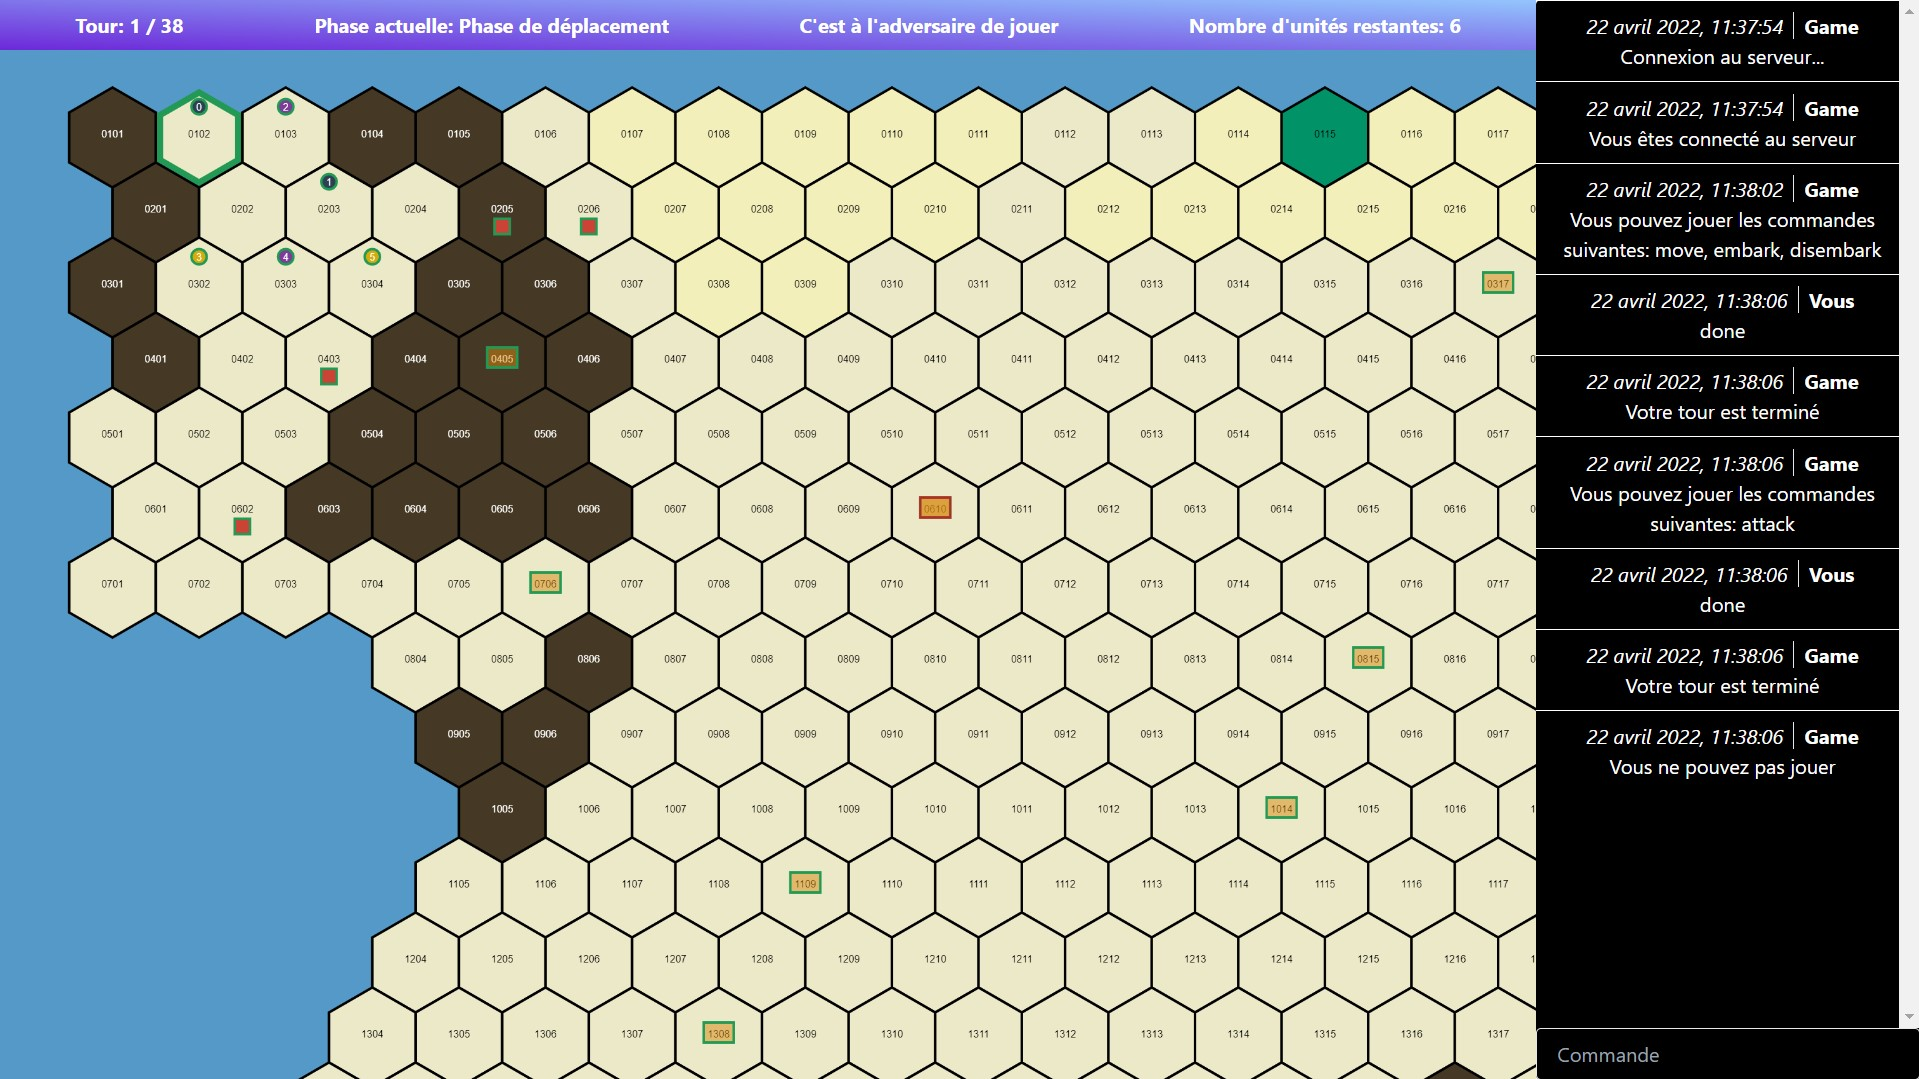
\includegraphics[scale=0.35]{data/fin_tour.jpg}
    \caption{Fin du tour pour le joueur 1}.
    \label{fig:fin_tour}
\end{figure}




\subsection{Tests}
\newpage


\begin{center}
    \begin{tabular}{|l|l|l|}
        \hline

        n° & test                                      & sortie attendu                                                    \\ \hline
        \multicolumn{3}{|c|}{srcfolder}                                                                                    \\
        \hline
        1  & Vérifier les fichiers dans le dossier src & Ils devraient tous être des fichiers .ts dans src/main            \\
        2  &                                           & Ils devraient tous être des fichiers .ts  ou  .json dans src/test \\
        3  &                                           & Les fichiers contenant la classe doivent être en majuscules       \\
        \hline
        \multicolumn{3}{|c|}{index}                                                                                        \\
        \hline
        4  & Game map test                             & Instancier la carte                                               \\
        5  &                                           & L'hexagone valide ne doit pas lancer                              \\
        6  &                                           & Hex invalide devrait jeter                                        \\
        \hline
        \multicolumn{3}{|c|}{SocketsServer}                                                                                \\
        \hline
        7  & Test socket server                        & initialise socket serveur                                         \\
        8  &                                           & WebServer stocke correctement clientPort                          \\
        9  &                                           & WebServer stocke correctement serverPort                          \\
        10 &                                           & Démarre webserver                                                 \\
        11 &                                           & Initialise le joueur 1 et la connexion                            \\
        12 &                                           & Initialise le joueur 2 et la connexion                            \\
        13 &                                           & Essaye de connecter un 3ième joueur                               \\
        14 &                                           & Le jeu devrait être lancé                                         \\
        15 &                                           & Le jeu devrait avoir player1                                      \\
        16 &                                           & Le jeu devrait avoir player2                                      \\
        17 &                                           & Le jeu devrait avoir le joueur 1 avec la bonne prise              \\
        18 &                                           & Le jeu devrait avoir le joueur 1 avec la bonne prise              \\
        19 &                                           & Seul le joueur 2 devrait rester                                   \\
        20 &                                           & La connexion joueur 1 devrait redémarrer une nouvelle partie      \\
        21 &                                           & La déconnexion de joueur 2 devrait arrêter le jeu                 \\
        22 &                                           & La connexion joueur 2 devrait redémarrer une nouvelle partie      \\
        23 &                                           & joueur 1 peut envoyer un ping au serveur                          \\
        24 &                                           & Le joueur 1 envoie un message au joueur 2                         \\
        25 &                                           & fermer le serveur                                                 \\



        \hline
    \end{tabular}


    \begin{tabular}{|l|l|l|}

        \hline
        \multicolumn{3}{|c|}{StateMachine}                                                                     \\
        \hline

        26 & Test de la machine d'état    & Test d'initialisation                                              \\
        27 &                              & Réinitialise la machine d'état                                     \\
        28 &                              & Test  de la phase de transitions                                   \\




        \hline
        \multicolumn{3}{c}{GameInstance}                                                                       \\
        \hline
        29 & Test d'instance du jeu       & Initialise le serveur                                              \\
        30 &                              & Initialise joueur  1                                               \\
        31 &                              & Initialise joueur 2                                                \\
        32 &                              & Le jeu doit démarrer                                               \\
        33 &                              & Obtient les unités du joueur 1                                     \\
        34 &                              & Obtient les unités du joueur 2                                     \\
        35 &                              & Le premier joueur déplace une unité valide                         \\
        36 &                              & Le premier joueur ne parvient pas à déplacer une unité inexistante \\
        37 &                              & Le premier joueur ne parvient pas à se déplacer                    \\ %vers un hexagone non existant \\
        38 &                              & Le premier joueur essaie de déplacer l'unité d'un adversaire       \\
        39 &                              & Passer au joueur suivant                                           \\
        40 &                              & Ferme le serveur                                                   \\


        \hline
        \multicolumn{3}{c}{Player}                                                                             \\
        \hline
        41 & Test Player                  & Player doit être correcte                                          \\
        42 &                              & Test hasUnit                                                       \\
        43 &                              & Le Dump est correct et supprimez les Dump                          \\


        \hline
        \multicolumn{3}{c}{AbstractUnit}                                                                       \\
        \hline

        44 & Test des unités est correcte & Unit doit être correcte                                            \\
        45 &                              & Le dé est correcte                                                 \\
        46 &                              & le JSON est correcte                                               \\

        \hline
        \multicolumn{3}{c}{Bases}                                                                              \\
        \hline

        47 & Base doit être correct       & Base envoie                                                        \\
        48 &                              & Base reçoit                                                        \\
        49 &                              & Réinitialise la Base                                               \\
        50 &                              & Place la Base                                                      \\

        \hline
        \multicolumn{3}{c}{Game}                                                                               \\
        \hline
        51 & Tests de Game                & Initialise le jeu                                                  \\
        52 &                              & le jeu devrait montrer les unités disponibles pour se déplacer     \\
        53 &                              & le jeu vérifie correctement les fournitures                        \\
        54 &                              & vérifications embarquer                                            \\
        55 &                              & vérifications débarquement                                         \\
        \hline
        \multicolumn{3}{c}{Pathfinder}                                                                         \\
        \hline
        56 & Test Pathfinder              & renvoie le coût en points de mouvement                             \\ %Le poids renvoyé doit être le coût en points de mouvement et trouve le chemin le plus court \\
        57 &                              & Ne traverse pas ou n'entre pas dans l'hex ennemi                   \\
        \hline
        \multicolumn{3}{c}{CombatSimulator}                                                                    \\
        \hline
        58 & Test  simulateur de combat   & Les résultats de moral doivent être corrects                       \\
        59 &                              & Les résultats des dommages doivent être corrects                   \\
        \hline
    \end{tabular}
\end{center}
